\documentclass[conference]{IEEEtran}
\IEEEoverridecommandlockouts
% The preceding line is only needed to  funding in the first footnote. If that is unneeded, please comment it out.
\usepackage{cite}
\usepackage{amsmath,amssymb,amsfonts}
\usepackage{algorithmic}
\usepackage{graphicx}
\usepackage{textcomp}
\usepackage{xcolor}
\def\BibTeX{{\rm B\kern-.05em{\sc i\kern-.025em b}\kern-.08em
		T\kern-.1667em\lower.7ex\hbox{E}\kern-.125emX}}
\begin{document}
	
	\title{"Roots + GloVe" for arabic sentiment Analysis \\
		%{\footnotesize \textsuperscript{*}Note: Sub-titles are not captured in Xplore and
	}
	%\thanks{Identify applicable funding agency here. If none, delete this.}
	%}
	
	
	\author{\IEEEauthorblockN{1\textsuperscript{st} Given Name Surname}
		\IEEEauthorblockA{\textit{dept. name of organization (of Aff.)} \\
			\textit{name of organization (of Aff.)}\\
			City, Country \\
			email address or ORCID}
		\and
		\IEEEauthorblockN{2\textsuperscript{nd} Given Name Surname}
		\IEEEauthorblockA{\textit{dept. name of organization (of Aff.)} \\
			\textit{name of organization (of Aff.)}\\
			City, Country \\
			email address or ORCID}
		\and
		\IEEEauthorblockN{3\textsuperscript{rd} Given Name Surname}
		\IEEEauthorblockA{\textit{dept. name of organization (of Aff.)} \\
			\textit{name of organization (of Aff.)}\\
			City, Country \\
			email address or ORCID}
		\and
		\IEEEauthorblockN{4\textsuperscript{th} Given Name Surname}
		\IEEEauthorblockA{\textit{dept. name of organization (of Aff.)} \\
			\textit{name of organization (of Aff.)}\\
			City, Country \\
			email address or ORCID}
		\and
		\IEEEauthorblockN{5\textsuperscript{th} Given Name Surname}
		\IEEEauthorblockA{\textit{dept. name of organization (of Aff.)} \\
			\textit{name of organization (of Aff.)}\\
			City, Country \\
			email address or ORCID}
		\and
		\IEEEauthorblockN{6\textsuperscript{th} Given Name Surname}
		\IEEEauthorblockA{\textit{dept. name of organization (of Aff.)} \\
			\textit{name of organization (of Aff.)}\\
			City, Country \\
			email address or ORCID}
	}
	
	\maketitle
	
	\begin{abstract}
		Sentiment analysis of social media has been widely investigated by many researchers in several languages. Despite the tremendous amount of data generated on Arabic social media, researches in this language still lack. In literature, many approaches were used to deal with Arabic sentiment analysis, among them machine learning, which use word vector representations to train models. The big challenge in this approach is the huge volume and the sparsity of the matrix representation. This paper is dedicated to present a new hybrid solution to tackle these two problems. The proposed Arabic sentiment analysis combines a newly bag of roots (BoR) technique and global vector distributional representations (GloVe). The obtained system is evaluated using two classifiers support vector machine (SVM) and logistic regression (LR), with three well-known datasets in the literature. It yields encouraging results in terms of precision, recall and F1-score and considerable reducing of time processing where compared with others approaches cited in literature.
	\end{abstract}
	
	\begin{IEEEkeywords}
		sentiment Analysis, Roots, GloVe, word vector representations , Machine learning
	\end{IEEEkeywords}
	
	\section{Introduction}
	Sentiment analysis of social media (SASM) is one of the most active research areas in this last decade. Millions of words are written in few seconds in different topics on these platforms. This massive amount of data has attracted researchers and companies to study this content. The basic idea of sentiment analysis is to predict and classify feelings from comments or tweets as positive, negative or neutral \cite{7351837}.
	Various techniques have been used to deal with sentiment analysis; we noticed from the- state-of-the-art, that there exist three main approaches: lexicon-based\cite{8673428}, machine learning\cite{8392100} and hybrid model\cite{8250273}. The idea of lexicon-based approaches is based on the text polarity obtained according to the polarities of words that compose it. The machine learning techniques use two datasets for training and test. A training set is used by a classifier to learn the differentiating features of texts, while a test dataset is used to verify the classifier performance, others researchers indicate that hybridization of both the machine learning and the lexicon-based approaches improve sentiment classification performance.
	Although machine learning approach achieves good results in several languages, in Arabic is still relative due to the complex morphology and the huge numbers of terms in Arabic language where we count more than 13 million words \cite{8067771}. Hence, most of the researchers have applied several techniques to reduce this huge amount of terms \cite{8098736} \cite{8500193}; among the recent techniques in the literature, the distributional representations (GloVe \cite{8324059}, Word2Vec \cite{8480191}, FastText \cite{8258460}), which use context to create the vectors.
	
	In our paper, we propose a hybrid Arabic sentiment analysis, where we introduce a roots module in the Global vector representations (GloVe) to reduce the numbers of words. We chose roots of words because in Arabic language there are rarely words with opposite polarities that have the same root, which is not suitable for other languages such as English and French that have a lot of words with the same root and opposite polarities, For instance, “Like and dislike”, “worth and worthless.” the main purpose is to improve the accuracy of the SA system and reducing the processing time  by compacting the vector space representations, which is the features used to create models. Our system is evaluated over two ML classifiers: Support vector Machine (SVM)\cite{6289583}, Logistic regression (LR)\cite{8284501}.  
	
	The remainder of this paper is organized as follow: the second section describes the existing related work in the literature. In Section 3 we present the GloVe distributional representations model. proposed approach and methodology employed to extract polarities from tweets. In Section 4, we explore the proposed approach and methodology employed to extract polarities from tweets. Finally, we present the experiments and discuss the results of the system evaluated over two Datasets used several metrics, and finally concluding remarks and perspective are given.
	
	
	\section{Related Work}
	
	
	In the last years, Arabic Sentiment analysis has become an attractive research. Several approaches are conducted in   this area. The main approaches found in literature:  Lexicon Based, Machine Learning or Hybrid models. 
	
	The Lexicon based use the polarity of words to determine texts sentiments. Authors of \cite{8549704} and \cite{7975223} use SentiWordNet and SentiStrength 3.0 respectively. They are English bag of words that use Machine Translation from Arabic to English; they didn’t give good results due to the difficulty of Arabic words, which are characterized by multiple meanings. Furthermore, the authors in [\cite{8125054} established a standard of Arabic lexicon was (Ar-SenL). It’s a large set of Arabic words embedding. There are no perfect accessible Arabic sentiment lexicons. Hence, several researchers used their own lexicons created in a defined field area such as EL-Beltagy \cite{6544421}, who interested in Egyptian Dialect.
	
	The Machine Learning approach is based mostly on the notion of supervised learning technique. The ML's main idea is to split the dataset into a learning set and a set of tests, learning the first pre-labeled subset to create a model, and then testing the result with the second subset. In the literature, most of ML techniques are used in the English language, but still lack in Arabic. In \cite{8530517}, authors have used: Decision Tree and SVM algorithms to predict sentiments. In \cite{7514636}, authors used different classifiers such as SVM, RBF to classify the polarity tweets collected from different domains. 
	
	The hybrid approach, uses Machine learning and Lexicon Based. There is few works in Arabic language. In \cite{8250273} authors proposed hybrid approach of Arabic tweets sentiment analysis, in their method, the lexical-based classifier used to label the training data and the output is utilized to train the SVM machine learning classifier.
	In \cite{8706408} authors, have used hybrid approach for sentiment analysis in Arabic tweets based on the deep learning model with features weighting.
	\section{GloVe For Arabic sentiment Analysis}
	In literature, there are several models available for distributional word representations; these models are based on the linguistic hypothesis "Words that occurs in the same context tends to have the same meaning." They are unsupervised techniques, which use statistics and probabilities of word occurrence in huge corpora.
	
	Global vector representation (GloVe) is a famous one of the space vector representation.  It is developed by Pennington et al, (2014) \cite{8318770}, which aim to learn low-dimensional vector representations of terms. The global idea of GloVe is the use of ratios of co-occurrence probabilities instead of word occurrence. The formula of glove is denoted in the Equation 1, while $w_{i}$ ,  $w_{j}$,  $w_{k}$ are three words and  $p_{ik}$ the probability of  $w_{k}$ being the context word of  $w_{i}$, then if the ratios of   $p_{ik}$ and  $p_{jk}$ is closer to 1, the representations of   $w_{i}$ ,  $w_{j}$ are similar, else should be far away from  $w_{k}$.
	
	\begin{equation}
	F((w_{i}-w_{j})^Tw_{k}) =\frac{P_{ik}}{P_{jk}}\label{Pr}
	\end{equation}
	
	The use of GloVe model in the sentiment analysis system had improved the accuracy and reduced the dimensionality of matrix representations. The basic workflow of GloVe for sentiment analysis comprises three phases as shown in Figure1 which is illustrated below. In the first, word vector representation is learnt from a big corpus such as Wikipedia by the use of GloVe model. In the second phase, after the preprocessing of tweets or comments collected from the benchmark datasets, a list of words is created. In the third step, words are compared with the vectors created from the first step and get their representations, to be used as features for machine learning classifiers in order to create models.
	\begin{figure}[htbp]
		\centerline{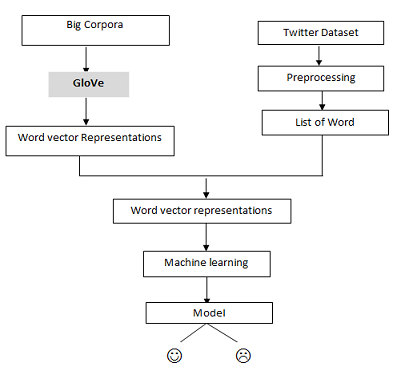
\includegraphics[scale=0.9]{GloveSA.png}}
		\caption{The Glove model for sentiment analysis scheme.}
		\label{fig}
	\end{figure}
	Although that GloVe representation gives better results in sentiment analysis in several languages such as English, French and Spanish languages than classical model such as bags of words (BoG), in Arabic language is still poor due to the hard structure and morphology of The Arabic texts and numbers of words that exceeds the thirteen million. To enhance the results and make gives the Glove representation more benefit to Arabic languages we added new module in the basic scheme of sentiment analysis, called roots extraction module (REM), it will be explained in the next section.
	
	\section{Our Approach}
	The purpose of this paper is to create a system that extracts sentiments from tweets, using a new approach, which is based on combining roots and GloVe word embedding to create efficient and reduced features to use it in machine learning classifiers. The system is illustrated in Figure 2.
	
	\begin{figure}[htbp]
		\centerline{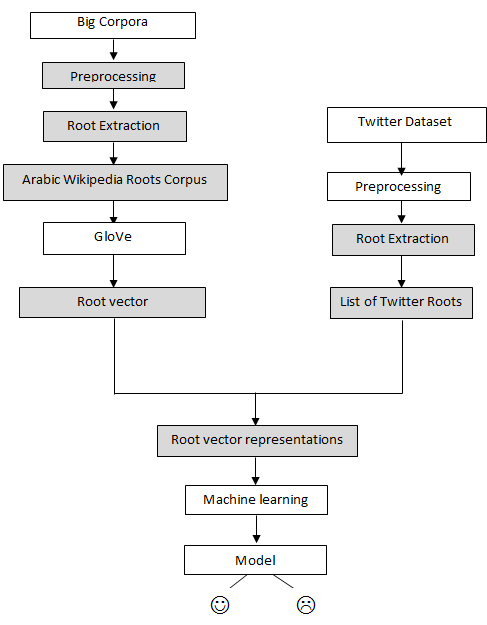
\includegraphics[scale=0.70]{RootGloveSA.png}}
		\caption{Combine of Roots and The Glove model for sentiment analysis scheme.}
		\label{fig}
		
	\end{figure}
	Similar as the basic Glove sentiment analysis scheme, our system contains three phases. The novel in this scheme is the roots extraction model, which we used in the phase one and two. In the first phase, a preprocessing step has been performed to clean and remove stops and meaningless words, then an efficient root extraction approach is applied to construct a Wikipedia roots corpus, finally in this phase, we applied the GloVe model to learn the root vector representations. In the second phase, after the preprocessing of tweets collected from the benchmark datasets, the root extraction module is applied to create a list of roots; after, roots are compared with the root vectors created in the first step and get their representations, to be used as features in the third phase for machine learning classifiers in order to create models.
	
	\section{Experements and Results}
	In this section, we describe the two experiments realized and their results concerned the accuracy of our Arabic sentiment analysis system. All codes are implemented in python, we used also the package glove-python which is available online to implement the Glove model. 
	
	As mentioned in section 4, we used three data collection, one collected from Arabic Wikipedia a huge corpus necessary to applied GloVe to create the word vector representation using context to compact the size of matrix representations. 
	
	Two well-known dataset collected from twitter, RES1 Dataset of restaurant reviews scrapped from qaym.com 8364 reviews , Book reviews from the website Goodreads, with 16448 tweets . (see Table1).
	To create models, two efficient classifiers are used, support vector machine (SVM), an approach widely used in different languages due to the effectiveness in result of texts classification. This algorithm use portion of the dataset to training step then test will be doing by remaining part . The second is logistic regression (LR), which is one from log-linear family classifier. It’s a probabilistic algorithm used in binary classification, it is a discriminative classifier .
	
	In the experiments, parameter of has arbitrary chosen, for the GloVe model, the vector size was fixed to 300 and windows size to 3, while for the classifiers we use the standard parameters, and datasets are divided to 70\% for training and 30\% for the test.
	
	\begin{table}[!ht]
		\large        %% not "\fontsize{12}{12}\selectfont"
		\caption{DATASETS.}\label{label}
		\centering    %% not "\center{...}"
		\begin{tabular}{|c|c|}
			\hline
			Dataset&Total Reviews\\     %% no "&" at start of row
			\hline
			RES1&8364 tweets\\
			\hline
			BOOK REVIEWS&16448 tweets\\
			\hline
			
		\end{tabular}
	\end{table}
	
	We used the confusion matrix as shown in Table 2 and three metrics to evaluate the three classifiers (Precision, Recall and F-measure).
	
	\begin{table}[!ht]
		\large        %% not "\fontsize{12}{12}\selectfont"
		\caption{Confusion Matrix.}\label{label}
		\centering    %% not "\center{...}"
		\begin{tabular}{|c|c|c|}
			\hline
			&P(predicted)&N (predicted)\\     %% no "&" at start of row
			\hline
			P (actual)&True Positive&False Positive\\
			\hline
			N (actual)&False Positive&True Positive\\
			\hline
			
		\end{tabular}
	\end{table}
	
	
	Precision: provides from positive classified sentiment, how many are actually positive? It’s calculated in use of True positive and False Positive with the Equation 2.
	
	\begin{equation}
	precision =\frac{True Positive}{True Positive + False Positive}\label{Pr}
	\end{equation}
	
	Recall: indicates from actual positive sentiment, how many are classified as positive? To compute it two parameters are used True positive and False Negative with the Equation 3.
	
	\begin{equation}
	Recall =\frac{True Positive}{True Positive + False Negative}\label{Re}
	\end{equation}
	
	F1- score is calculated in use of Precision and Recall with the Equation 4.
	
	\begin{equation}
	F1-Score =\frac{2*precision*Recall}{Precision + Recall}\label{F1}
	\end{equation}
	\subsection{System evaluation over SVM and LR classifiers with RES1 dataset:}\label{AA}
	The dataset RES1 contains 8364 tweets,   applying the classifiers: (SVM) and (LR) give Confusion Matrix and metrics shown below in Table 3 and illustrated in Figure 3:
	
	\begin{table}[!ht]
		\large        %% not "\fontsize{12}{12}\selectfont"
		\caption{RES1 Dataset with the Classifiers results.}\label{label}
		\centering    %% not "\center{...}"
		\begin{tabular}{|c|c|c|}
			\hline
			RES1 Dataset&SVM&LR\\     %% no "&" at start of row
			\hline
			TP&1064&1086\\
			\hline
			FP&190&196\\
			\hline
			TN&144&108\\
			\hline
			FN&269&299\\
			\hline
			Precision&0.8484&0.8471\\
			\hline
			recall&0.7981&0.7841\\
			\hline
			F1score&0.8224&0.8143\\
			\hline
		\end{tabular}
	\end{table}
	
	\begin{figure}[htbp]
		
		\centerline{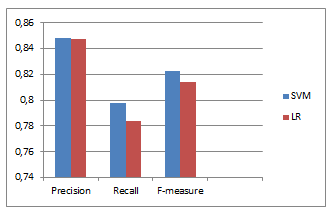
\includegraphics{fig3.png}}
		\caption{Result of the classifiers on RES1.}
		\label{fig}
	\end{figure}
	\subsection{System evaluation over SVM and LR classifiers with BOOK REVIEW dataset:}\label{AA}
	The dataset BOOK REVIEW contains 16448 tweets, applying the classifiers: (SVM) and (LR) give Confusion Matrix and metrics shown below in Table 4 and illustrated in Figure 4:
	
	
	\begin{table}[!ht]
		\large        %% not "\fontsize{12}{12}\selectfont"
		\caption{BOOK REVIEW  Dataset with the Classifiers results.}\label{label}
		\centering    %% not "\center{...}"
		\begin{tabular}{|c|c|c|}
			\hline
			BOOK REVIEW Dataset&SVM&LR\\     %% no "&" at start of row
			\hline
			TP&1308&1331\\
			\hline
			FP&298&298\\
			\hline
			TN&358&355\\
			\hline
			FN&1326&1326\\
			\hline
			Precision&0.7851&0.7989\\
			\hline
			recall&0.8144&0.8170\\
			\hline
			F1score&0.7995&0.8078\\
			\hline
		\end{tabular}
	\end{table}
	
	\begin{figure}[htpb]
		
		\centerline{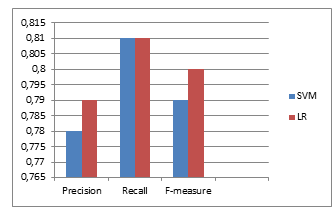
\includegraphics{fig4.png}}
		\caption{Result of the classifiers on BOOK REVIEW.}
		\label{fig}
		
	\end{figure}
	\subsection{Coparison of results with GloVe model without Roots on the two datasets:}\label{AA}
	
	\subsection{Results and Discussion:}\label{AA}
	
	
	\section{Conclusion}
	
	\bibliographystyle{IEEEtran}
	
	
	\bibliography{IEEEabrv,../references/ref01}
	
\end{document}
